\subsubsection{Spannungsverstärkung}
Die Werte zur Bestimmung der Spannungsverstärkungen wurden bei einer
Eingangsspannung von $U_{\mathrm{RMS}} = 100 \, \si{\milli\volt}$ und einer
Frequenz von $f_e = 1 \, \si{\kilo\hertz}$ bestimmt. Der Lastwiderstand wurde
von $100 \, \si{\kilo\ohm}$ bis $1 \, \si{\kilo\ohm}$ variiert. Die
Spannungsverstärkungen bei den jeweiligen Lastwiderstandswerten ist dann
der Quotient aus Ausgangs- und Eingangsspannung. Die Spannungswerte wurden
als RMS-Werte am Oszilloskop gemessen. Der interne Lastwiderstand beträgt $R_{\mathrm{L,intern}} =
100 \, \si{\kilo\ohm}$.


\begin{table}[H]
  \begin{center}
    \begin{tabular}{|c|c|c|c|}
      \hline
      $U_e / \si{\milli\volt}$ & $U_a / \si{\milli\volt}$ & $R_{\mathrm{L,gesamt}} / \si{\kilo\ohm}$ & $V_u$\\
      \hline
      \hline
      99.92 & 1080 & 100 & 10.81\\
      99.95 & 1050 & 33.33 & 10.51\\
      99.93 & 954.5 & 9.09 & 9.55\\
      99.99 & 475.4 & 0.99 & 4.76\\
      \hline
    \end{tabular}
  \end{center}
  \caption{RMS-Spannungswerte und daraus resultierende Verstärkung bei
    verscheidenen Lastwiderständen (ohne $R_3$)}
\end{table}

\begin{figure}[H]
  \begin{center}
    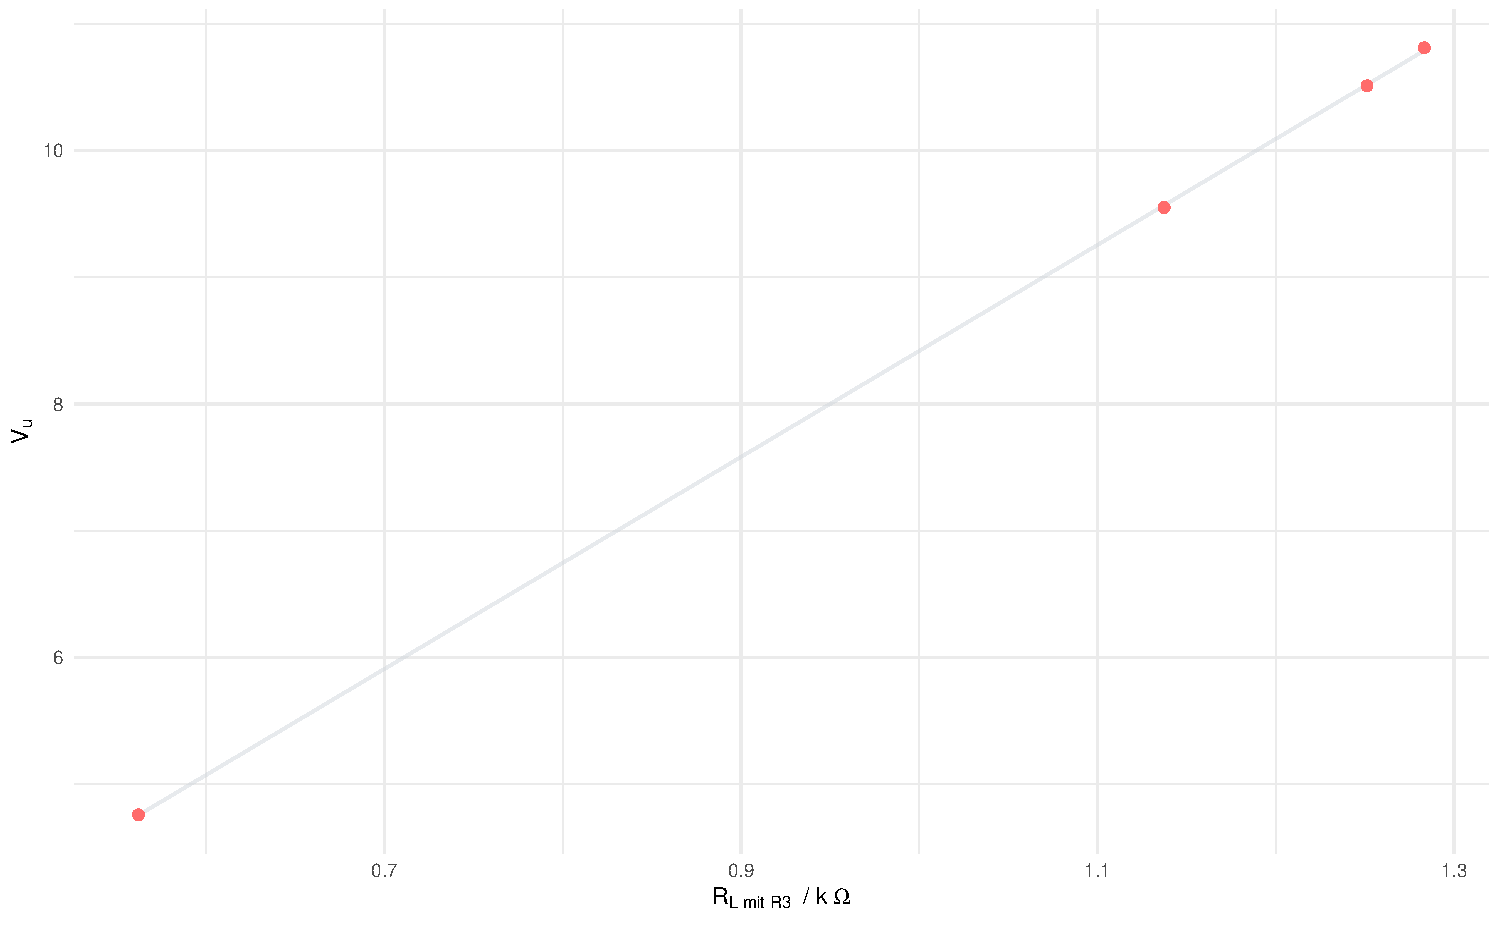
\includegraphics[width=\textwidth]{2_4/2_4_1_R3.pdf}
  \end{center}
  \caption{Graph der Messwerte, $R_3$ berücksichtigt}
\end{figure}

Der Zusammenhang zwischen Lastwiderstand und Verstärkung ist dem der vorherigen
Schaltung (ESIGK1) ähnlich. Die theoretische Steilheit des Transistors im Arbeitspunkt ist hier
\[g_{m,\mathrm{theoretisch}} = \frac{I_C}{U_T} = \frac{5.23 \, \si{\milli\ampere}}{26 \,
    \si{\milli\volt}} = 201.154 \, \si{\milli\siemens}\]

Durch die Gegenkopplung der Ausgangs- auf die Eingangsspannung wird, wie der
Versuch bestätigt, die Verstärkung der Emitterschaltung deutlich verringert.

\subsubsection{Eingangswiderstand}
Der Eingangswiderstand wurde auch hier nach der $U/2$-Methode bestimmt.

$U_{a0} = 1.08 \, \si{\volt}$
$U_{a1} = 500 \, \si{\milli\volt}$

Der dabei ermittelte Widerstandswert ist
\[r_e = 11 \, \si{\kilo\ohm}\]

Aus dem Datenblatt:
\[r_\pi = 0.9 \, \si{\kilo\ohm}\]
\[r_0 = 33.33 \, \si{\kilo\ohm}\]

Der theoretische Widerstandswert ist
\[r_{e} = R_2 // ((1+B_N) \cdot (R_5 // r_0) + r_\pi) = 21.35 \, \si{\kilo\ohm}\]

Der theoretische Wert ist etwa das Doppelte des theoretischen Wertes,
möglicherweise ist ein Rechen- oder Messfehler aufgetreten.

\subsubsection{Ausgangswiderstand}
Der Ausgangswiderstand wurde wie in 2.3.3 aus Messung zweier Spannungswerte
ermittelt. Der externe Ausgangslastwiderstand ist $R_L = 10 \, \si{\kilo\ohm}$

\[U_{a0} = 1080 \,\si{\milli\volt}\]
\[U_{a1} =  954.5 \,\si{\milli\volt}\]

\[r_a = 10 \, \si{\kilo\ohm} \left( \frac{1080 \, \si{\milli\volt}}{954.5 \,
      \si{\milli\volt}} -1 \right) \approx 1.3 \, \si{\kilo\ohm}\]



